\documentclass[a4paper, 12pt]{article}
\usepackage[utf8]{inputenc}
\usepackage{graphicx}
\usepackage{fancyhdr}
\usepackage{lipsum}
\usepackage{fix-cm}  
\usepackage{bophook}
\usepackage{tikz}
\usepackage{roboto}
\usepackage{minted}
\usepackage{pdflscape}
\usepackage{xcolor}
\usepackage{newverbs}
\usepackage{parskip} % http://ctan.org/pkg/parskip
\usepackage[nottoc,numbib]{tocbibind} %add bib to table of contents
\usepackage{hyperref}
% to avoid table floats, use with \FloatBarrier
\usepackage{placeins}
% table merge cells
\usepackage{multirow}
\usepackage[normalem]{ulem}
\useunder{\uline}{\ul}{}



\hypersetup{
colorlinks=true,
allcolors = black,
urlcolor = [rgb]{0,0,0.8},
}



% logo fib
% \AtBeginPage{
% \begin{tikzpicture}[remember picture,overlay]
%   \node[anchor=north east,inner sep=10pt] at (current page.north east)
%               {
\includegraphics[scale=0.2]{images/upc-fib-logos.png}};
% \end{tikzpicture}
% }


% https://tex.stackexchange.com/a/141128

%%%%% OLD SOLUTION %%%%%
% \definecolor{codegrey}{rgb}{0.937, 0.937, 0.937}

% \newverbcommand{\code}
%   {\begin{lrbox}{\verbbox}}
%   {\end{lrbox}\colorbox{codegrey}{\box\verbbox}}

\usepackage{fancyvrb,newverbs,xcolor}
\usepackage{lipsum}% just for this example

\definecolor{cverbbg}{gray}{0.93}

\newenvironment{cverbatim}
 {\SaveVerbatim{cverb}}
 {\endSaveVerbatim
  \flushleft\fboxrule=0pt\fboxsep=.5em
  \colorbox{cverbbg}{\BUseVerbatim{cverb}}%
  \endflushleft
}
\newenvironment{lcverbatim}
 {\SaveVerbatim{cverb}}
 {\endSaveVerbatim
  \flushleft\fboxrule=0pt\fboxsep=.5em
  \colorbox{cverbbg}{%
    \makebox[\dimexpr\linewidth-2\fboxsep][l]{\BUseVerbatim{cverb}}%
  }
  \endflushleft
}

\newcommand{\ctexttt}[1]{\colorbox{cverbbg}{\texttt{#1}}}
\newverbcommand{\code}
  {\setbox\verbbox\hbox\bgroup}
  {\egroup\colorbox{cverbbg}{\box\verbbox}}


%\pagestyle{fancy}

\makeatletter
\newcommand\HUGE{\@setfontsize\Huge{60}{70}}
\makeatother    


\graphicspath{ {./images/} }
\bibliographystyle{unsrt}

%%%%% DOCUMENT %%%%%

\begin{document}
\setlength{\parskip}{10pt}
\setlength{\parindent}{0pt}


\begin{titlepage}
\definecolor{title-red}{HTML}{cc0000}

\center 

\Large
Polytechnic University of Catalonia

\vspace{.5cm}
\large


\textit{Checkpoint delivery}

\roboto
\vspace*{1cm}
\HUGE
\textcolor{title-red}{OpenSlicer}

\vspace{0.5cm}

\LARGE
A portable three-dimensional object slicer

\vspace{1cm}


\normalsize \textit{Author} \\ \large{Luuk Willemsen} \\ \vspace{0.5cm}
\normalsize \textit{Director} \\ \large{Marta Fairén} \\ \vspace{0.5cm}
% \normalsize \textit{GEP Tutor} \\ \large{Marcos Eguiguren}


\vspace{2cm}

\normalsize
\today

\vspace{3cm}



\includegraphics[width=1\textwidth]{images/fib-upc.png}
\end{titlepage}

\tableofcontents
\pagebreak

%%%%%%%%%%%%%%%%%%%%%%%%%%%%%%%%%%%%%%%%%%%%%%%%%%%%%%
%%%%%%%%%%%%%%%%%%%%%%%%%%%%%%%%%%%%%%%%%%%%%%%%%%%%%%
%%%%%%%%%%%%%%%%%%%%%%%%%%%%%%%%%%%%%%%%%%%%%%%%%%%%%%
\section{Context and scope}

\subsection{Introduction}
\subsubsection{Project goal}
There are multiple techniques to create real-world objects from a three-dimensional model.
We will focus on Fused Filament Fabrication, a specific form of 3D printing, which consists in melting a filament of thermoplastic polymer, in a layer-by-layer fashion.

When modeling 3D objects with computer programs, they are usually represented as a triangle mesh (for example, in \textsc{stl} format). A 3D printer can only execute simple commands, such as moving a motor forward, or extruding filament. These commands are usually in \textsc{gcode} format.

Slicing is the process of converting the 3D model as a triangle mesh to the \textsc{gcode} required by the 3D printer. A 3D printer typically has a simple microcontroller that is not powerful enough to slice the model, so an external program, called a \textsc{slicer} is used.

It is useful for 3D printer owners to remotely monitor and control it, stop it in case of a failure, and even start a print while not being present. This is usually accomplished by connecting a small computer to the printer. These computers  are able to slice a model, but often have limited resources, difficult processor architectures, or the process is very slow.

To solve this, we create \textsc{OpenSlicer}. A slicer that is designed to run in a web browser, so it is platform independent. Since the slicing occurs in the client's browser, the slicer can easily be hosted as a static page on the 3D printer itself.


\subsubsection{Stakeholders}
\begin{itemize}
    \item \textbf{Project developer}. I will be developing the project, doing the necessary research, testing and programming to make it succeed.
    \item \textbf{Project director}. Marta Fairén is the director of this project. As an Associate Professor of the Computer Science department of the Polytechnic University of Catalonia, she will be helping the project developer with any problems, as well as providing feedback, improvement suggestions and technical advice to make sure the project succeeds.
    \item \textbf{The community} will be able to contribute, learn, improve, share, and use the software.
    \item \textbf{3D printer owners}  will be able to use the slicer from their phones or laptops to remotely slice their objects and print them.
    \item \textbf{3D printer manufacturers} will be able to host the slicer on the printer directly, without having to worry about updates, or maintenance of the slicer. They can then focus only on their main business: building 3D printers.
\end{itemize}

%%%%%%%%%%%%%%%%%%%%%%%%%%%%%%%%%%%%%%%%%%%%%%%%%%%%%%
%%%%%%%%%%%%%%%%%%%%%%%%%%%%%%%%%%%%%%%%%%%%%%%%%%%%%%
%%%%%%%%%%%%%%%%%%%%%%%%%%%%%%%%%%%%%%%%%%%%%%%%%%%%%%
\subsection{State of the art}
In this section we will briefly discuss existing technology, as well as what this project aims to accomplish.

\subsubsection{3D viewers}
3D visualization of models is a deeply explored field, and is used in all kinds of software: games, design studios, CAD programs, medical applications, etc. There are many robust libraries that offer 3D visualization, like DirectX, Metal or OpenGL. These libraries however are very low level, and too tedious to work with for our purpose. Instead, we will use \textbf{three.js} \cite{gh:threejs}, a high-level 3D visualization library for the web.

\subsubsection{Polygon clipping}
There are numerous clipping libraries in different languages \cite{gh:clipper-lib, gh:clipper, gh:lineclip}. This field has been deeply explored in the past, and efficient polygon clipping is considered a solved problem. We will use \textbf{clipper-lib} for polygon clipping.

\subsubsection{Slicers}
Some slicers already exist in the literature \cite{gh:curaengine, gh:slic3r}. However, there are no slicers in JavaScript. Therefore, this project will use mostly own algorithms but some will be inspired on existing slicers or ports of well-known slicing algorithms for other language.

\subsubsection{Bridging the gap}
Existing slicers are designed for optimal performance, and are compiled to run as a binary on the user's system. We compromise performance, as our slicer will run in the browser, but obtain the following advantages:

\begin{itemize}
    \item A 3D printer's microcontroller can serve the slicer without the need of a more powerful computer.
    \item Slicing on mobile phones and tablets
    \item Refreshing the page will update the slicer.
    \item Browser based, so cross platform by nature
    \item No dependencies or installs.
    \item Possibility to run in the cloud and manage 3D models from any device.
\end{itemize}

Most of these features are new for Fused Filament Fabrication slicers. There is a performance overhead of running the software in a browser, but it is compensated for by a possible cloud-based slicing engine (if we decide to monetize this idea), and by the availability on all platforms.






%%%%%%%%%%%%%%%%%%%%%%%%%%%%%%%%%%%%%%%%%%%%%%%%%%%%%%
%%%%%%%%%%%%%%%%%%%%%%%%%%%%%%%%%%%%%%%%%%%%%%%%%%%%%%
%%%%%%%%%%%%%%%%%%%%%%%%%%%%%%%%%%%%%%%%%%%%%%%%%%%%%%
\subsection{Scope}
A fully functional slicer will be developed and tested on a live 3D printer. The slicer should be able to output \textsc{gcode} that produces a physical object that accurately resembles the original 3D model.

\subsubsection{Minimum requirements}
There are several stages to the slicing process that must be implemented for it to work properly:

\begin{itemize}
    \item \textbf{A graphical user interface} to move, scale and rotate the object, as well as manipulating different settings of the slicing process, such as the speed, layer height, nozzle diameter, print and bed temperature.
    \item \textbf{A 2-manifold \cite{wiki:2-manifold} check algorithm}, that detects whether the input model is watertight and can be sliced correctly.
    \item \textbf{A 3D geometry intersection algorithm}, that generates layer perimeter polygons intersecting a plane with the model's triangles.
    \item \textbf{A 2D polygon clipping algorithm} to generate internal perimeters and calculate the infill.
    \item \textbf{An ordering algorithm} to create a chain of segments that will form each layer in the final print. This should minimize the total print time.
    \item \textbf{An output  generator}, that will take the segment chain and convert it to \textsc{gcode} for printing. This generator might also add calibration, homing, or other instructions at the begin or end of the gcode.
\end{itemize}

\subsubsection{Extras}

Additional features that greatly improve print quality, but are harder to implement may be added if time permits:

\begin{itemize}
    \item \textbf{Infill pattern generation}, to avoid printing at 100\% density.
    \item \textbf{Automatic support structure generation}, to be able to print with overhangs correctly.
    \item \textbf{Decimation}, to allow extremely detailed objects to be sliced correctly.
    \item \textbf{Retraction}, to improve bridging and reduce stringing.
    \item \textbf{Layer-by-layer settings} can greatly improve surface finish while keeping print times low.
\end{itemize}


%%%%%%%%%%%%%%%%%%%%%%%%%%%%%%%%%%%%%%%%%%%%%%%%%%%%%%
%%%%%%%%%%%%%%%%%%%%%%%%%%%%%%%%%%%%%%%%%%%%%%%%%%%%%%
%%%%%%%%%%%%%%%%%%%%%%%%%%%%%%%%%%%%%%%%%%%%%%%%%%%%%%
\subsection{Possible obstacles and solutions}
This section will discuss some of the problems that might arise during the development of the project.

\begin{itemize}
    \item \textbf{Breaking the 3D printer} would leave us without a testing machine. This is a realistic problem because sending the wrong \textsc{gcode} to the printer may run the nozzle into the bed, or heat it so much that the power supply fails.
    \item \textbf{Floating point precision}. The precision of floating points or doubles is limited, so we will need to find a solution to that. There are several ways to do this, which will be discussed in the technical part of this project.
    \item \textbf{Bugs.} Developing a slicer is not an easy task. Companies have been developing them for decades and their commercial products are still containing a lot of bugs. It seems natural that our team consisting of a single developer will have some trouble designing a fully functional slicer from scratch and will encounter some time-consuming bugs that might lead to delays or even missed deadlines. We will use a version control system and continuous integration tests to track bugs and prevent them from happening in the first place.
    \item \textbf{Algorithm efficiency}. It is entirely possible that the algorithms developed during this project are not fast enough to run on decent hardware. If this is the case the project might fail completely, or be too slow to be usable. The solution to this problem is to ensure that we are using reasonably fast algorithms.
\end{itemize}

%%%%%%%%%%%%%%%%%%%%%%%%%%%%%%%%%%%%%%%%%%%%%%%%%%%%%%
%%%%%%%%%%%%%%%%%%%%%%%%%%%%%%%%%%%%%%%%%%%%%%%%%%%%%%
%%%%%%%%%%%%%%%%%%%%%%%%%%%%%%%%%%%%%%%%%%%%%%%%%%%%%%
\subsection{Methodology and rigor}

\subsubsection{Methodology}
Since there will be a single developer in the project, it does not make sense to follow very complex methodologies, but we will apply some good practices and principles from well-known methodologies:
\begin{itemize}
    \item From \textbf{Test Driven Development}: We will have automated tests before every commit to avoid introducing most bugs.
    \item From \textbf{Agile Development} We will only commit code that compiles and runs correctly, and make small changes.
    \item We will set some milestones in order to be aware of the general timeline of the project.
    \item Using git as version control system will allow us to go back to any previous state of the project, as well as to rapidly track down bugs using git-bisect \cite{git-bisect}
\end{itemize}

\subsubsection{Rigor}
\begin{itemize}
    \item To check whether our project meets industry standards we will benchmark the different stages of the slicing process.
    \item We will exhaustively test edge cases and difficult objects in order to validate the robustness of our slicer. This will be done in an automated fashion as well as by hand.
    \item Real 3D prints will be used to measure the accuracy of the slicer, absolute and relative errors will be measured and improved on.
\end{itemize}



\section{Project planning}
\subsection{Schedule}

\subsubsection{Estimated duration}
The work required for this project, including development, documentation, possible bugs and fixes, is approximately 4 months.

All possible issues mentioned in deliverable 1 are taken into account when designing this planning. However, during project development it might be possible that the proposed planning is altered.

\subsection{Task description}

This project has a lot of different modules that are independent from each other in functionality, but some might require the output of a previous module before being able to work properly. The planning is important to follow, so we do not break time dependencies between the modules.

\subsubsection{Initial 3D Viewer and GUI}
We will use \emph{three.js} as a base for the 3D viewer and will work on top of it. It's fairly easy to set up and show any 3D model in the viewer, as it's one of the basic examples included in the library. We then need some functions to rotate, scale, translate and otherwise manipulate the object. I have some experience with three.js, so this task should last no longer than a week. This task requires the use of the mentioned library, as well as an IDE. We will use WebStorm \cite{webstorm} for the development of the project and all of it's components.

\subsubsection{Slicer}
Sharing the name with the overall process, in this case the slicing algorithm will only be responsible for obtaining a polygon for a given height. This module will be called multiple times in order to slice the whole object.

\subsubsection{Toolpath generator}
After the slicer has generated a polygon, this module will be responsible for generating a set of lines in an internal format that will be used by the \emph{GCODE} generator later on.

\subsubsection{GCODE generator}
Once we have our toolpath generated, we need to convert it to a language the 3D Printer understands: GCODE. This module is responsible for the conversion and the final output of the program. This task requires a 3D printer or simulator to test the generated output.



\subsubsection{Resources}

The following resources are required in order to complete the previous and tasks.

\begin{itemize}
    \item All modules require \emph{human resources} to develop the required code.
    \item A computer to develop with.
    \item A 3D printer or simulator to test the output of the slicer.
    \item A place for the developer to work
    \item All the mentioned software
\end{itemize}


\subsection{Time estimation}
An estimation of the project's timeline is shown in \autoref{table:task-time}. Times are approximate but should account for most possible changes and delays.

\FloatBarrier
\begin{table}[h!]
\centering
\begin{tabular}{ |c|c| } 
    \hline
    Task & Estimated duration (h)  \\ 
    \hline
    
    \hline
    GEP & 75  \\ 
    \hline
    Project setup & 20  \\ 
    \hline
    3D Viewer & 40  \\ 
    \hline
    GUI & 25  \\ 
    \hline
    Slicer & 80  \\ 
    \hline
    Toolpath generator & 80  \\ 
    \hline
    GCODE generator & 80  \\ 
    \hline
    Bugfixes and improvements & 50 \\
    
    \hline
    Total & 450 \\
    \hline
\end{tabular}
\caption{Estimated time for each task}\label{table:task-time}
\end{table}
\FloatBarrier


Every task or module will have several stages. We will need to read through existing examples and projects to get a general idea of what to do. Then we will need to decide the implementation details, implement the module, test it and fix any possible bugs.

\subsubsection{Gantt chart}

\autoref{fig:gantt-chart} shows a more detailed overview of the task planning in a Gantt chart. The timeline may change slightly due to project requirements or unexpected bugs. This is accounted for in the final stage of the project, bugfixes and improvements. More on this in the next section.


\begin{figure}[H]
    \noindent\makebox[\textwidth]{
        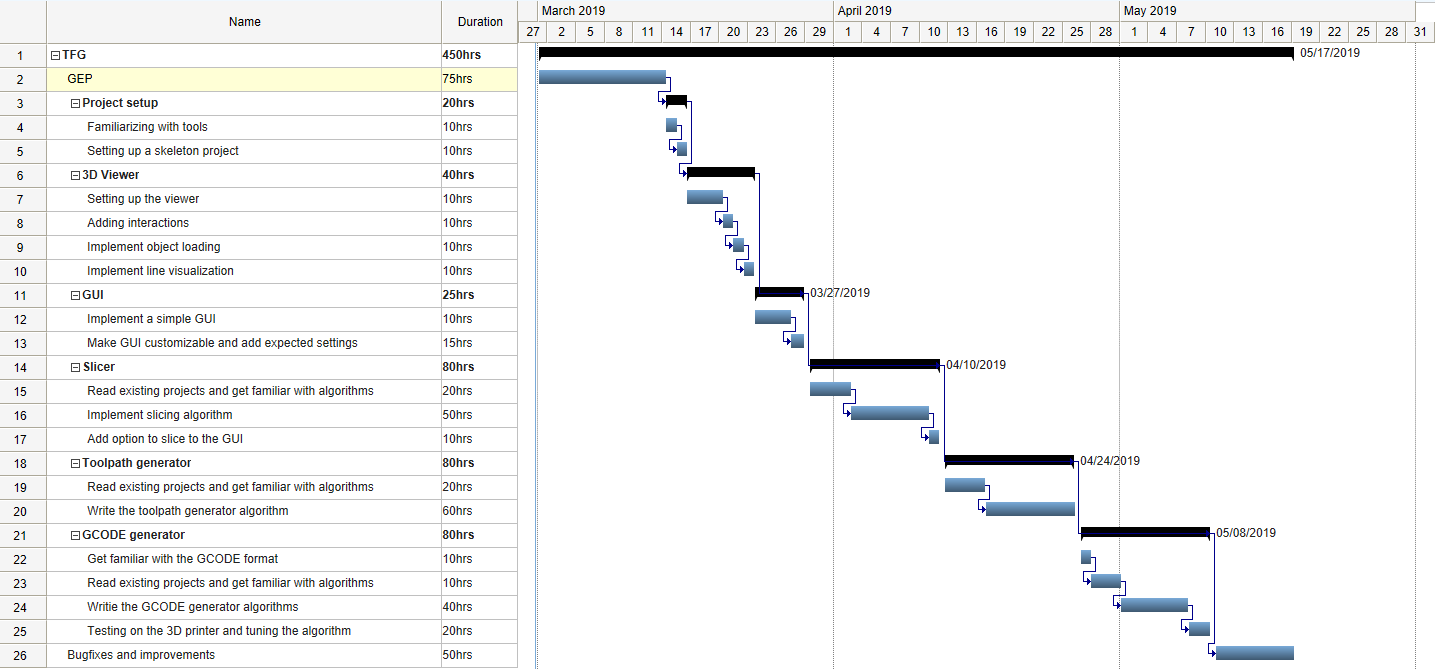
\includegraphics[width=1.3\textwidth]{images/gantt.png}
    }
    \caption{Gantt chart of the project. Generated with Gantter \cite{gantter}}
    \label{fig:gantt-chart}
\end{figure}


\subsection{Alternatives and action plan}

In the previous delivery we mentioned the methodologies that will be used, including Test Driven Development, and heavy use of git. This should reduce the risk of bugs and accelerate the development quality as well as the speed.

We have a total workload of 450 hours, with a dedication 40 hours per week. Extra time is given at the end to account for possible bugs or potential problems and slowdowns, which are discussed in the previous delivery.

The 50 hours of bug fixes and improvements are not necessarily at the end. Instead they are distributed throughout the project. In case of a problem, the complete focus will be on solving it as soon as possible, and this time will be deducted from the bug fix time at the end. Any time left at the end will be used for improvements.

Particular detailed are discussed as follows:

\subsubsection{Breaking the 3D printer}
We will mitigate the risk of breaking the 3D printer by running wrong gcode on it by simulating it first. Slic3r and Cura both have a gcode viewer, so we can verify that the generated output is correct (or at least it won't move to negative coordinates, or outside of the build area). In case the printer ends up breaking, we have an alternative, cheaper 3D printer available for testing.

\subsubsection{Floating point precision}
Floating point precision may not be enough for some geometry operations. In these rare cases, the model will still be sliced correctly, but will have some features or some missing detail. This is a limitation of all slicers, and it is possible to still get those detail, but no current slicer does this so we consider this beyond the scope of this project.

\subsubsection{Bugs}
We already discussed multiple times how we will deal with possible bugs. In particular, whenever a bug is found, we will write a test case that reproduces the bug, and use git bisect to find the exact commit where the bug was introduced. Since we are also making small commits with specific changes, it will be easy to find out what the cause of the bug was and how to fix it.

\subsubsection{Algorithm efficiency}
Some of the slowest algorithms are already handled by libraries, but we still need to find efficient algorithms for slicing, polygon generation and toolpath generation. We have assigned extra time to each of these module's planned time to account for finding efficiency improvements. Since most slicers are able to run on slow hardware, it is very likely that every algorithm will be possible to implement with acceptable efficiency. Alternatively we can accept slower algorithms that will still produce a decent running time, although it will be noticeable to the user.

\section{Budget and sustainability}
\subsection{Project budget}
In this section, an estimation of the cost of the project is presented, taking into account the previously mentioned resources.

\subsubsection{Hardware budget}

\autoref{table:res-hw}
shows the hardware resources budget needed in order to develop and test the project.

\FloatBarrier
\begin{table}[h!]
\centering
\begin{tabular}{ |c|c|c|c|c| } 
    \hline
    Product & Price & Units & Useful life & Amortization \\
    \hline
    \hline
    Apple MacBook Pro & 2000€ & 1 & 8 years & 250€ \\ 
    \hline
    Prusa i3 MK3 3D Printer & 769€ & 1 & 4 years & 192.25€ \\ 
    \hline
    \hline
    Total & 2769€ & & & 442.25€ \\
    \hline
\end{tabular}
\caption{Hardware budget}\label{table:res-hw}
\end{table}
\FloatBarrier

\subsubsection{Software budget}

\autoref{table:res-sw}
shows the software resources budget needed in order to develop and test the project.

\FloatBarrier
\begin{table}[h!]
\centering
\begin{tabular}{ |c|c|c|c| } 
    \hline
    Product & Price & Useful life & Amortization \\
    \hline
    \hline
    Git & 0€ & & 0€ \\ 
    \hline
    GitHub & 0€ & & 0€ \\ 
    \hline
    macOS High Sierra & 0€ & & 0€ \\ 
    \hline
    Google Chrome browser & 0€ & & 0€ \\ 
    \hline
    Gantter & 0€ & & 0€ \\ 
    \hline
    Slic3r & 0€ & & 0€ \\ 
    \hline
    Slic3r PE & 0€ & & 0€ \\ 
    \hline
    Ultimaker Cura & 0€ & & 0€ \\ 
    \hline
    \LaTeX & 0€ & & 0€ \\ 
    \hline
    webpack & 0€ & & 0€ \\ 
    \hline
    WebStorm & 129€ & 1 year & 129€ \\ 
    \hline
    \hline
    Total & 129€ & & 129€ \\
    \hline
\end{tabular}
\caption{Software budget}\label{table:res-sw}
\end{table}
\FloatBarrier

\subsubsection{Human resources budget}

\autoref{table:res-hres}
shows the human resources budget needed in order to develop and test the project.

\FloatBarrier
\begin{table}[h!]
\centering
\begin{tabular}{ |c|c|c|c| } 
    \hline
    Role & Price/h & Hours & Cost \\
    \hline
    \hline
    Project manager & 50€ & 50 & 2,500€ \\
    \hline
    Software developer & 30€ & 300 & 9,000€ \\
    \hline
    Tester & 30€ & 100 & 3,000€ \\
    \hline
    \hline
    Total & & 450 & 14,500€ \\
    \hline
\end{tabular}
\caption{Human resources budget \cite{dev-salary, pm-salary, qa-eng-salary}}\label{table:res-hres}
\end{table}
\FloatBarrier

Since the modules of the project are mostly independent, and equally important, the different roles are distributed evenly across all tasks.

\subsubsection{Unexpected costs}
\autoref{table:res-extra} shows a generous budget margin for problems or deviations that may arise. This extra budget is very unlikely to be used because of the robust planning of the previous deliverable.

\FloatBarrier
\begin{table}[h!]
\centering
\begin{tabular}{ |c|c|c|c| } 
    \hline
    Role & Price/h & Hours & Cost \\
    \hline
    \hline
    Project manager & 50€ & 10 & 500€ \\
    \hline
    Software developer & 30€ & 20 & 600€ \\
    \hline
    Tester & 30€ & 10 & 300€ \\
    \hline
    \hline
    Total & & & 1,400€ \\
    \hline
\end{tabular}
\caption{Extra human resources budget \cite{dev-salary, pm-salary, qa-eng-salary}}\label{table:res-extra}
\end{table}
\FloatBarrier



\subsubsection{Direct costs breakdown}

\autoref{table:res-direct-breakdown} shows the breakdown of costs per task listed in the Gantt chart.



\FloatBarrier
\begin{table}[h!]
\centering
\begin{tabular}{ |c|c|c|c|c|c| } 
    \hline
    Task & HW & PM & SW Dev & Tester & Total \\
    \hline
    \hline
    Project Setup & 571.25€ & 250€ & 1500€ & 0€ & 1879€ \\
    \hline
    3D Viewer, GUI & 0€ & 500€ & 1500€ & 600€ & 2,600€ \\
    \hline
    Slicer & 0€ & 500€ & 1500€ & 600€ & 2,600€ \\
    \hline
    Toolpath generator & 0€ & 500€ & 1500€ & 600€ & 2,600€ \\
    \hline
    GCODE generator & 0€ & 500€ & 1500€ & 600€ & 2,600€ \\
    \hline
    Bugfixes & 0€ & 250€ & 1500€ & 600€ & 2,350€ \\
    \hline
    \hline
    Total & 571.25€ & 2,500€ & 9,000€ & 3,000€ & 15,071.25€ \\
    \hline
\end{tabular}
\caption{Direct costs breakdown}
\label{table:res-direct-breakdown}
\end{table}
\FloatBarrier


\subsubsection{Indirect costs}

\autoref{table:res-indirect-costs}
shows the indirect costs related to developing and testing the project.

For this project we will fix the price of electricity at 0.12€/kWh \cite{price-electricity-endesa}. A 3D printer consumes about 0.2kWh, a laptop about 0.06kWh, and the rest (router, lights) about 0.03kWh. We will assume everything is running during the whole development of the project, except for the 3D printer, which will only be needed in the latest stages of the project, and we will consider it is used only the last 50\% of the project. This brings us at a total electricity consumption of about 100kWh.

\FloatBarrier
\begin{table}[h!]
\centering
\begin{tabular}{ |c|c|c|c| } 
    \hline
    Product & Price & Amount & Cost \\
    \hline
    \hline
    Electricity & 0.12€/kWh & 100kWh & 12€ \\
    \hline
    Internet & 30€/month & 4 months & 120€ \\
    \hline
    Coffee and snacks & 10€/week & 16 weeks & 160€ \\
    \hline
    \hline
    Total & & & 292€ \\
    \hline
\end{tabular}
\caption{Indirect costs \cite{price-electricity-endesa, price-vodafone-adsl, price-coffee-nespresso}}\label{table:res-indirect-costs}
\end{table}
\FloatBarrier

\subsubsection{Total budget}
We will calculate the total budget by adding all previous budgets together. This is shown in \autoref{table:res-total-costs}.

\FloatBarrier
\begin{table}[h!]
\centering
\begin{tabular}{ |c|c| } 
    \hline
    Concept & Estimated cost \\
    \hline
    \hline
    Hardware & 442.25€ \\
    \hline
    Software & 129€ \\
    \hline
    Human resources & 14,500€ \\
    \hline
    Unexpected costs & 1,400€ \\
    \hline
    Indirect costs & 292€ \\
    \hline
    \hline
    Total & 16,763.25€ \\
    \hline
\end{tabular}
\caption{Total budget}\label{table:res-total-costs}
\end{table}
\FloatBarrier

\subsubsection{Budget management}
It is unlikely that we will exceed our budget, since our project planning section was quite robust. We have already accounted for a generous error margin to fix bugs or compensate for delays in the development of complex algorithms. It might still be possible to need extra resources or hire an additional software developer as a consultant. We have also taken this into account when creating our budget. We are being extremely cautious about human resources budget allocation since this is the most expensive part of it.

As we discussed earlier, it is possible to break the 3D printer while doing our testing. In this case we will work on a gcode simulator that comes with most existing slicers. This will add nothing to our budget, and we will continue the project in a theoretical way, without actual 3D printed tests or examples.

We will be monitoring the progress of the project according to the Gantt chart shown previously. If delays occur, we will allocate an extra software developer or tester to solve the specific issue that is causing the delay. In this case, this extra developer will count against the extra budget we have defined earlier.

Following the previous procedure, we can guarantee that we will not exceed our timeline significantly, and we will still stay in our allocated budget, since we already accounted for possible delays or unexpected costs.


\subsection{Sustainability report}


In this section we analyze the sustainability of the project. Its impact is analyzed in its three dimensions: social, economical and environmental.

This is a project consisting of mostly software. There are alternatives already in the market with similar features. We will not be causing a significant social, economical or environmental impact.

Sustainability does not really apply to this project in all of its dimensions, but we will analyze them anyway for the sake of completeness.

\subsubsection{Social impact}
On a personal level, this project allows me to push my limits on development and testing, as well as to deduce complex algorithms and development methods. It will help me know my limits and capabilities and provide me with a fun time to learn and experiment.

To the end user, this project does not have a significant social impact, since it is only a tool to convert solid models to 3D printer instructions.


\subsubsection{Economical impact}
We have already discussed and quantified the budget of this project in terms of hardware, software, and human resources. 

We try to use mostly free software, and our product will also be a free software tool. Existing free software slicers exist already, so this project will not make a big economical impact on the end user.


\subsubsection{Environmental impact}
We will be using 100kWh of electricity while developing and testing the project, which is equivalent to approximately 28.3 kg of CO${_2}$. This might seem like a lot until we add our team of humans, who breathe during development, which accounts for approximately 50 more kg of CO${_2}$, for a total of 78.3 kg \cite{co2-breathing}.


We will be using Polylactic Acid (PLA) as our only plastic during the testing phase. It is a bio-plastic material, biodegradable and reduces CO$_{2}$ \cite{pla-co2, env-impact-3dp}. This is one of the best materials to use when 3D printing and we choose this for our testing because of its nice environmental properties.


\subsubsection{Sustainability Matrix}
Taking into account the previous sections, in \autoref{table:sustainability-matrix} we show the sustainability matrix of this project in its three dimensions.

\FloatBarrier
\begin{table}[h!]
\centering
\begin{tabular}{|c|c|c|c|}
\hline
 & PPP & Useful Life & Risks \\ \hline
\multirow{2}{*}{Environmental} & \begin{tabular}[c]{@{}c@{}}Design\\ consumption\end{tabular} & \begin{tabular}[c]{@{}c@{}}Ecological\\ footprint\end{tabular} & \begin{tabular}[c]{@{}c@{}}Environmental\\ risks\end{tabular} \\ \cline{2-4} 
 & 9 / 10 & 18 / 20 & -5 / -20 \\ \hline
\multirow{2}{*}{Economical} & Bill & \begin{tabular}[c]{@{}c@{}}Viability\\ plan\end{tabular} & \begin{tabular}[c]{@{}c@{}}Economical\\ risks\end{tabular} \\ \cline{2-4} 
 & 8 / 10 & 17 / 20 & -2 / -20 \\ \hline
\multirow{2}{*}{Social} & \begin{tabular}[c]{@{}c@{}}Personal\\ impact\end{tabular} & \begin{tabular}[c]{@{}c@{}}Social\\ impact\end{tabular} & \begin{tabular}[c]{@{}c@{}}Social\\ risks\end{tabular} \\ \cline{2-4} 
 & 8 / 10 & 10 / 20 & -1 / -20 \\ \hline
\multirow{2}{*}{\begin{tabular}[c]{@{}c@{}}Sustainability\\ range\end{tabular}} & 25 / 30 & 45 / 60 & -8 / -60 \\ \cline{2-4} 
 & \multicolumn{3}{c|}{62 / 90} \\ \hline
\end{tabular}
\caption{Sustainability matrix}\label{table:sustainability-matrix}
\end{table}
\FloatBarrier



\break
\section{Legal}
\subsection{License}
Copyright 2019 Luuk Willemsen

Permission is hereby granted, free of charge, to any person obtaining a copy of this software and associated documentation files (the "Software"), to deal in the Software without restriction, including without limitation the rights to use, copy, modify, merge, publish, distribute, sublicense, and/or sell copies of the Software, and to permit persons to whom the Software is furnished to do so, subject to the following conditions:

The above copyright notice and this permission notice shall be included in all copies or substantial portions of the Software.

THE SOFTWARE IS PROVIDED "AS IS", WITHOUT WARRANTY OF ANY KIND, EXPRESS OR IMPLIED, INCLUDING BUT NOT LIMITED TO THE WARRANTIES OF MERCHANTABILITY, FITNESS FOR A PARTICULAR PURPOSE AND NONINFRINGEMENT. IN NO EVENT SHALL THE AUTHORS OR COPYRIGHT HOLDERS BE LIABLE FOR ANY CLAIM, DAMAGES OR OTHER LIABILITY, WHETHER IN AN ACTION OF CONTRACT, TORT OR OTHERWISE, ARISING FROM, OUT OF OR IN CONNECTION WITH THE SOFTWARE OR THE USE OR OTHER DEALINGS IN THE SOFTWARE.

\subsection{Laws and regulations}
This project is published as free software (see license section above) under a MIT license (or similar).

Since this is a software-only project, the above license covers all legal use of the software, and explicitly waives all liability and possible claims for the author. Users are responsible for any use of the software.


\section{Technical skills}
The technical skills that are considered relevant in this projects are the following, as per the project's initial presentation:

\begin{itemize}
    \item \textbf{CCO1.1}: 
    Evaluate the computational complexity of a problem, learn algorithmic strategies that can lead to its resolution, and recommend, develop and implement the one that guarantees the best performance in accordance with the established requirements. 
    \item \textbf{CCO2.3} Develop and evaluate interactive and complex information presentation systems, and their application to solving computer interaction design problems.
    \item \textbf{CCO2.6} Design and implement graphics, virtual reality, augmented reality and video games applications.
\end{itemize}


\pagebreak

\section{User Interface}
The User Interface consists of various components. In this section we will explain their functionality.

\subsection{3D Viewer}
We use \emph{three.js} as a \emph{WebGL} \cite{webgl} abstraction layer. This library is very well tested and makes it extremely easy to manipulate 3D objects. The included  \emph{OrbitControls} \cite{three:orbit-controls} allows for easy camera zooming, rotating and panning.

We will use the \emph{STL Loader} \cite{three:stl-loader}, to load any STL model as a three.js object, as shown in this \href{https://threejs.org/examples/?q=stl#webgl_loader_stl}{demo}.


\autoref{fig:viewer-demo} shows an example of the 3D Viewer with some basic models.

\begin{figure}[H]
    \noindent\makebox[\textwidth]{
        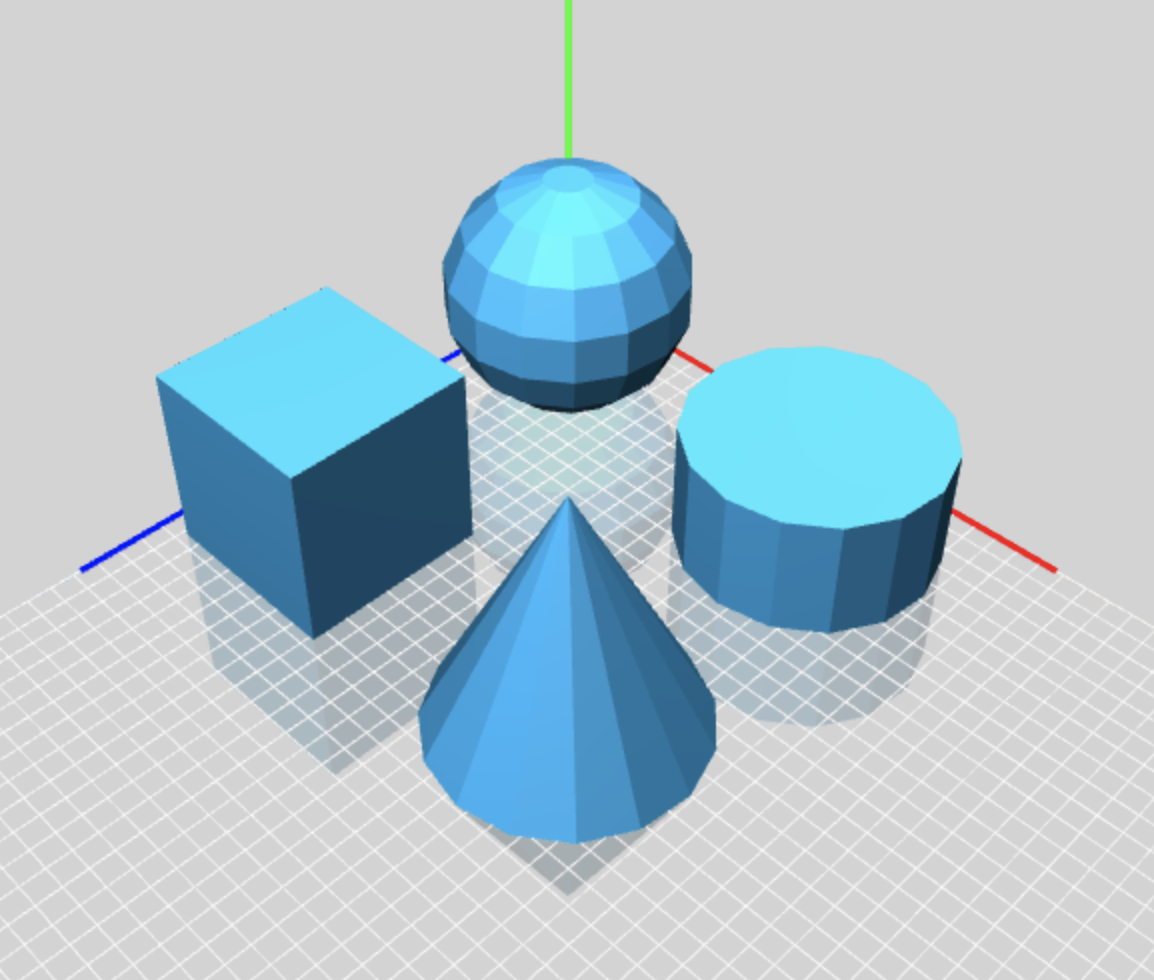
\includegraphics[width=.9\textwidth]{images/models.png}
    }
    \caption{3D Viewer example: Simple objects}
    \label{fig:viewer-demo}
\end{figure}


\subsection{GUI}
We will be using a 2D graphical user interface to allow the user to fine-tune the settings. This is important because of the great variety in 3D printer models that come in different sizes, have different speeds, materials, etc.

This GUI will control both printer-related settings (layer height, speed, temperature, etc), as well as the 3D Viewer (object color, rotation, translation, scale, etc).

We choose \emph{dat.GUI} \cite{dat.GUI} for its ease of use, as well as integrated save and load capabilities, that will make it easy to create presets for different printers or qualities. It supports boolean, range and color selectors, as well as actions and folders. This way we can organize the large amount of settings that we need for the project. 

\autoref{fig:dat.GUI} shows an example menu using dat.GUI with some of the settings that we will be implementing.

\begin{figure}[H]
    \noindent\makebox[\textwidth]{
        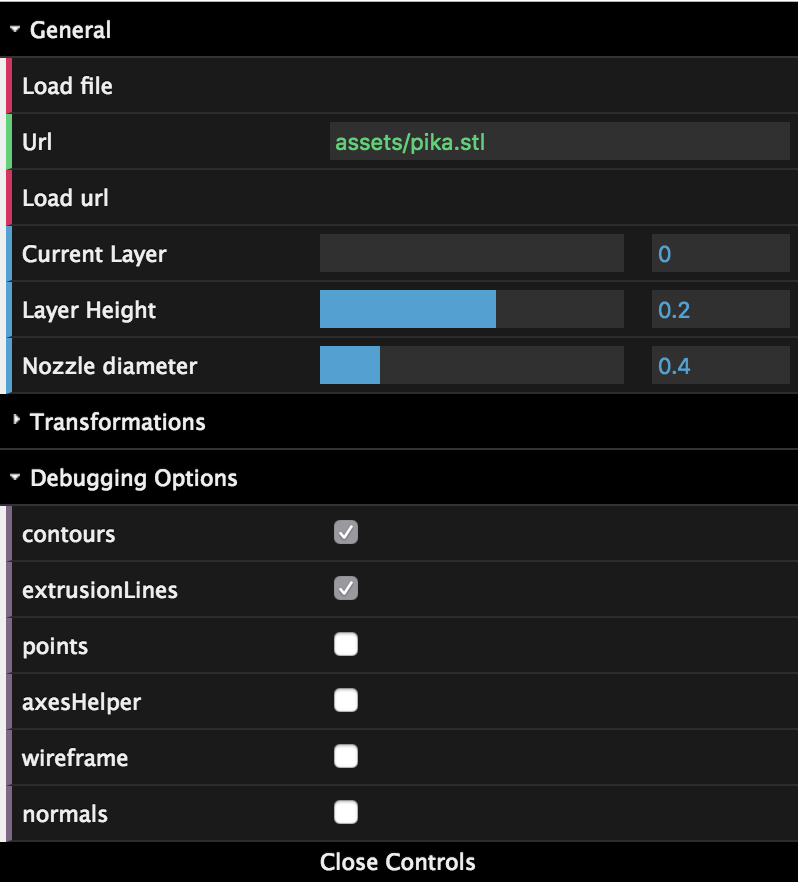
\includegraphics[width=.6\textwidth]{images/datgui.png}
    }
    \caption{dat.GUI: Sample menu}
    \label{fig:dat.GUI}
\end{figure}


Whenever the user changes a setting in the GUI, its \code|onChange()| method is called. dat.GUI also supports data binding, meaning that whenever the user interacts with the settings UI, the corresponding object property will be changed accordingly. We will use this to our advantage to simplify code.

To keep the GUI in the main scope, while keeping access to the data binding features, we will need to have the 3D Viewer communicate with the GUI. We will first create the 3D Viewer, and then pass it as a parameter to the GUI constructor. This ensures the GUI has access to the objects it needs to mutate, while reducing boilerplate code to a minimum. 

There will also be options that are not part of the 3D Viewer. For simplicity, we will be combining all configuration in an object called \code|Config|. This way we can save and restore all user preferences in a simple way.



\pagebreak

\section{Slicer}
The Slicer is responsible for taking an object as a list of triangles, and return a list of layers that the Toolpath Generator can later translate into GCODE. Each of these layers contains a list of ordered segments, which represent the path for the printing head to travel along.

The slicing process is much easier to understand and implement if done in parts.

\subsection{2-manifold checking}
To verify that the object is actually printable, we need to check that it is a valid 2-manifold. 

The initial plan was to test the validity of an object and rejecting non manifolds, but we have decided that it's best to just check and throw a warning in this case, and perform a slice on a best-effort basis. It is better to have an object slice wrong, than to not slice it at all.

Since this will only be a warning, it will be left out for now. In the final delivery it may or may not be included.

\subsection{Slicer}

It might be confusing to use the word Slicer for this part. Previously we defined slicing as the process of converting an object to 3D printer instructions. Slicing is also the process of cutting an object by a plane. This subsection is all about that: Intersecting a plane with a 3D object.

The algorithm we use for this is fairly simple: We simply take all triangles individually and intersect them with the plane. The intersection segment is added to the resulting list. If the plane intersects a given triangle on an edge or vertex, we will still include the segments in the result list. 

This algorithm will return an unordered list of segments, that are the segments where the plane intersects the object. If the object is a valid 2-manifold, then the resulting list can be ordered in a unique way, constructing a valid Surface.


\subsection{Polygon generator}
The polygon generation consists of taking the unordered list of segments that the Slicer produced, and order them into a surface.

We define a surfaces to be a list of polygons and a list of holes, which are also polygons. This definition of surface can describe any boolean 2D geometry.

Provided the object was a valid 2-manifold, all vertices in the slicer's output have degree exactly 2, which makes it trivial to construct the list of polygons.

We still need to determine whether a polygon is a hole or not. We can determine this easily with a simple ray tracing: Given a polygon, we take one of its vertices v and trace a straight line in any direction. If it intersects an odd number of polygons on one side of v, then this polygon is a hole. Otherwise it's part of the surface.

For this algorithm we need to be careful with edge cases: If we happen to trace a line from a hole, that intersects a parent polygon on one of its vertices, we might count that intersection twice, and think that this polygon is part of the surface while it's actually a hole.

\subsubsection{About the necessity of this section}
Instead of generating polygons for each layer, we can instead intersect the object directly with parallel lines for each desired height and width of the 3D printer. This will however generate only movement in one direction, and produces extremely ugly results, similar to when you color a drawing in a zigzag pattern instead of going around the edges first.

Having the polygon information allows us to create smaller versions of the polygons by perpendicularly insetting them by a fixed distance. This allows us to print the perimeters as a series of closed loops, and process the infill separately, without affecting the dimensions of the object, while also allowing for infill to be rectilinear.

In the final version of this document there will be pictures illustrating this process better.
\subsection{Generating segments}

Given a surface, we need to generate the actual segments along which the 3D printer will travel. To keep things simple, these will always be parallel lines, a fixed distance from each other.

We will follow a similar approach than with the slicing process: We will intersect each polygon with vertical planes to obtain the segments we want.

For each of those vertical planes, we intersect the polygon with it, and obtain a list of points. We sort these points and create segments between all adjacent points. We must get an odd number of segments, and all segments in even positions are holes, and are removed from the resulting set.

This gives us a list of segments that, if printed in the correct order, produce the expected object.


\subsection{Ordering segments}
Ordering segments is trivial. We will take a left-to-right and top-to-bottom approach to order them, which will yield relatively good results on any object. There are more complex ordering algorithms but they are out of the scope of this project.

\subsection{Toolpath generator}

The only thing that's left now is to translate the ordered segments into machine code. This is done by taking the start and end vertices of each segment and append the corresponding instructions to a list.








\section{Conclusions}

* TODO

\pagebreak

\begingroup
\raggedright
\bibliography{./src/references}
\endgroup

\end{document}
